\documentclass[11pt]{article}
\usepackage{geometry,tabularx,booktabs,float,natbib}                % See geometry.pdf to learn the layout options. There are lots.
\geometry{letterpaper}                   % ... or a4paper or a5paper or ... 
%\geometry{landscape}                % Activate for for rotated page geometry
%\usepackage[parfill]{parskip}    % Activate to begin paragraphs with an empty line rather than an indent
\usepackage{graphicx}
\usepackage{amssymb}
\usepackage{epstopdf}
\DeclareGraphicsRule{.tif}{png}{.png}{`convert #1 `dirname #1`/`basename #1 .tif`.png}
\newcommand{\myreferences}{references}

\title{Proposed Wrist-Mounted Smartdevice}
\author{Juan S. Carrillo}
%\date{}                                           % Activate to display a given date or no date

\begin{document}
\maketitle
\section{Introduction}
Wearables are growing in popularity. Recently, five out of the top ten crowdfunded campaigns on Kickstarter have been wearable devices. However, unlike the smartphone, it seems wearables have become more highly specialized, niche-specific products and fail to become standalone products in their own right. A large number of wrist-worn devices specialize as fitness trackers and do nothing more. More multipurpose products like Google Glass aren't completely independent; Google claims that in order for a ``great on-the-go Glass experience, it's essential to pair Glass to your phone or tablet." Overall, there are very few wearables that don't need to tether to a smartphone or other device in order to have full functionality. As a result it's very difficult for wearables to displace smartphones, which have much more functionality and just as much mobility as typical wearables. In this paper, I propose a device that combines the functionality of a smartphone with the mobility and wearability as a smartwatch.

\section{Background}
The functionality of wearables are greatly limited by their size and form. For example, head-mounted displays lack a graphical, direct manipulation oriented interface like touch screen smartphones. Tasks as simple as sending a text message on Google Glass is significantly more difficult than on a smartphone because a user would have to resort to voice recognition software, which is highly error prone and requires the user to be in an environment with very little background noise. Smartwatches have very small screens which limit the potential of incorporating touch screens into a smartphone. Some smartwatches use buttons to navigate their menus, but unfortunately this method also is unsatisfactory because it takes several button presses to navigate to specific tasks. The small size of wearables also limits their processing power as well as battery life. 

My design aims specifically to deal with issues and complaints common to smartwatches. The most important issue that I aim to address the ``fat finger problem". The fat finger problem is that smartwatches have relatively small screens compared to the size of our fingers. Several approaches such as iterative zooming, buttons, gestures, skin buttons, knobs and movable watch heads in order to compensate for the small screen Figure~\ref{fig:wearableApproaches}. However, I find these approaches unsatisfactory because they don't solve the fundamental problem of lacking space. Iterative zooming requires more taps and gestures to type in characters than a larger screen such as a cell phone or a tablet. Skin buttons make use of sensors that detect when a user a taps an icon illuminated on the users skin. Lighting conditions affect the effectivity of the sensors, and wearables should be equally effective regardless of the users setting. Buttons such as those included by the Pebble make it difficult for users to navigate a menu based system. Movable watch heads present moving parts which are often undesirable as they get worn over time.

\begin{figure}[H] %  figure placement: here, top, bottom, or page
   \centering
   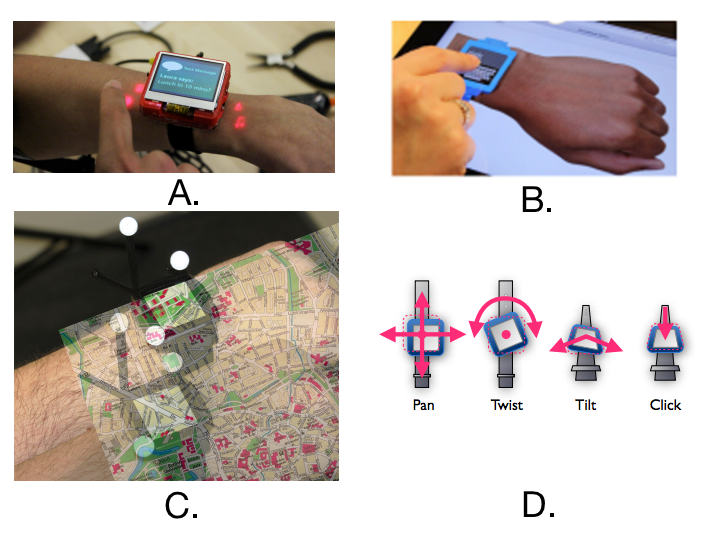
\includegraphics[width=5in]{wearableApproaches.png}       
   \caption{Different innovative interfaces for smartwatches, including Skin Buttons(A), ZoomBoard(B), Peephole Approach(C), and Movable Watch Heads(D)\cite{ZoomBoard,PeepholeWatch,tiltTwistSmartWatch, Skinbuttons}}
   \label{fig:wearableApproaches}
\end{figure}  

Of these approaches, the only one that attempts to increase the size of the interface is the skin buttons interface. I propose using a larger device with a larger, multitouch touchscreen. This solves the basic problems associated with tiny screens. My design borrows heavily from the design of smartphones, and I hope that the familiar design will appeal to users and allow usage of my device more intuitive and easy. Ultimately, the main advantage of a larger screen is that navigating the devices interface is much more easier. A larger device also allows for longer battery life and increased computational power. Admittedly, a larger device is also more obtrusive and more uncomfortable for users; I address these issues in another section of my paper.

\section{Physical Design}
I propose a wearable device that is worn on the user's forearm. It would be roughly five to six inches in length and would wrap around the forearm entirely. It would have two rigid, curved, durable sapphire multitouch touchscreen that would curve around the top and lower side of the forearm as in the diagram below, held together by a piece of hinged piece of material that locks into place on the other end of the screen section, as seen in Figure~\ref{fig:device}. This would allow the user to put on the device by sliding the device on to the inner forearm and then securing the device by locking it in place. 

The device has a single camera beneath the user's palm that acts front-facing camera when the user holds their arm with with the palm oriented towards the user's face, as seen in Figure~\ref{fig:deviceOnArm}. Additionally, by adjusting their arm, users can use this camera as back-facing camera in order to record images and videos. 
\begin{figure}[H] %  figure placement: here, top, bottom, or page
   \centering
   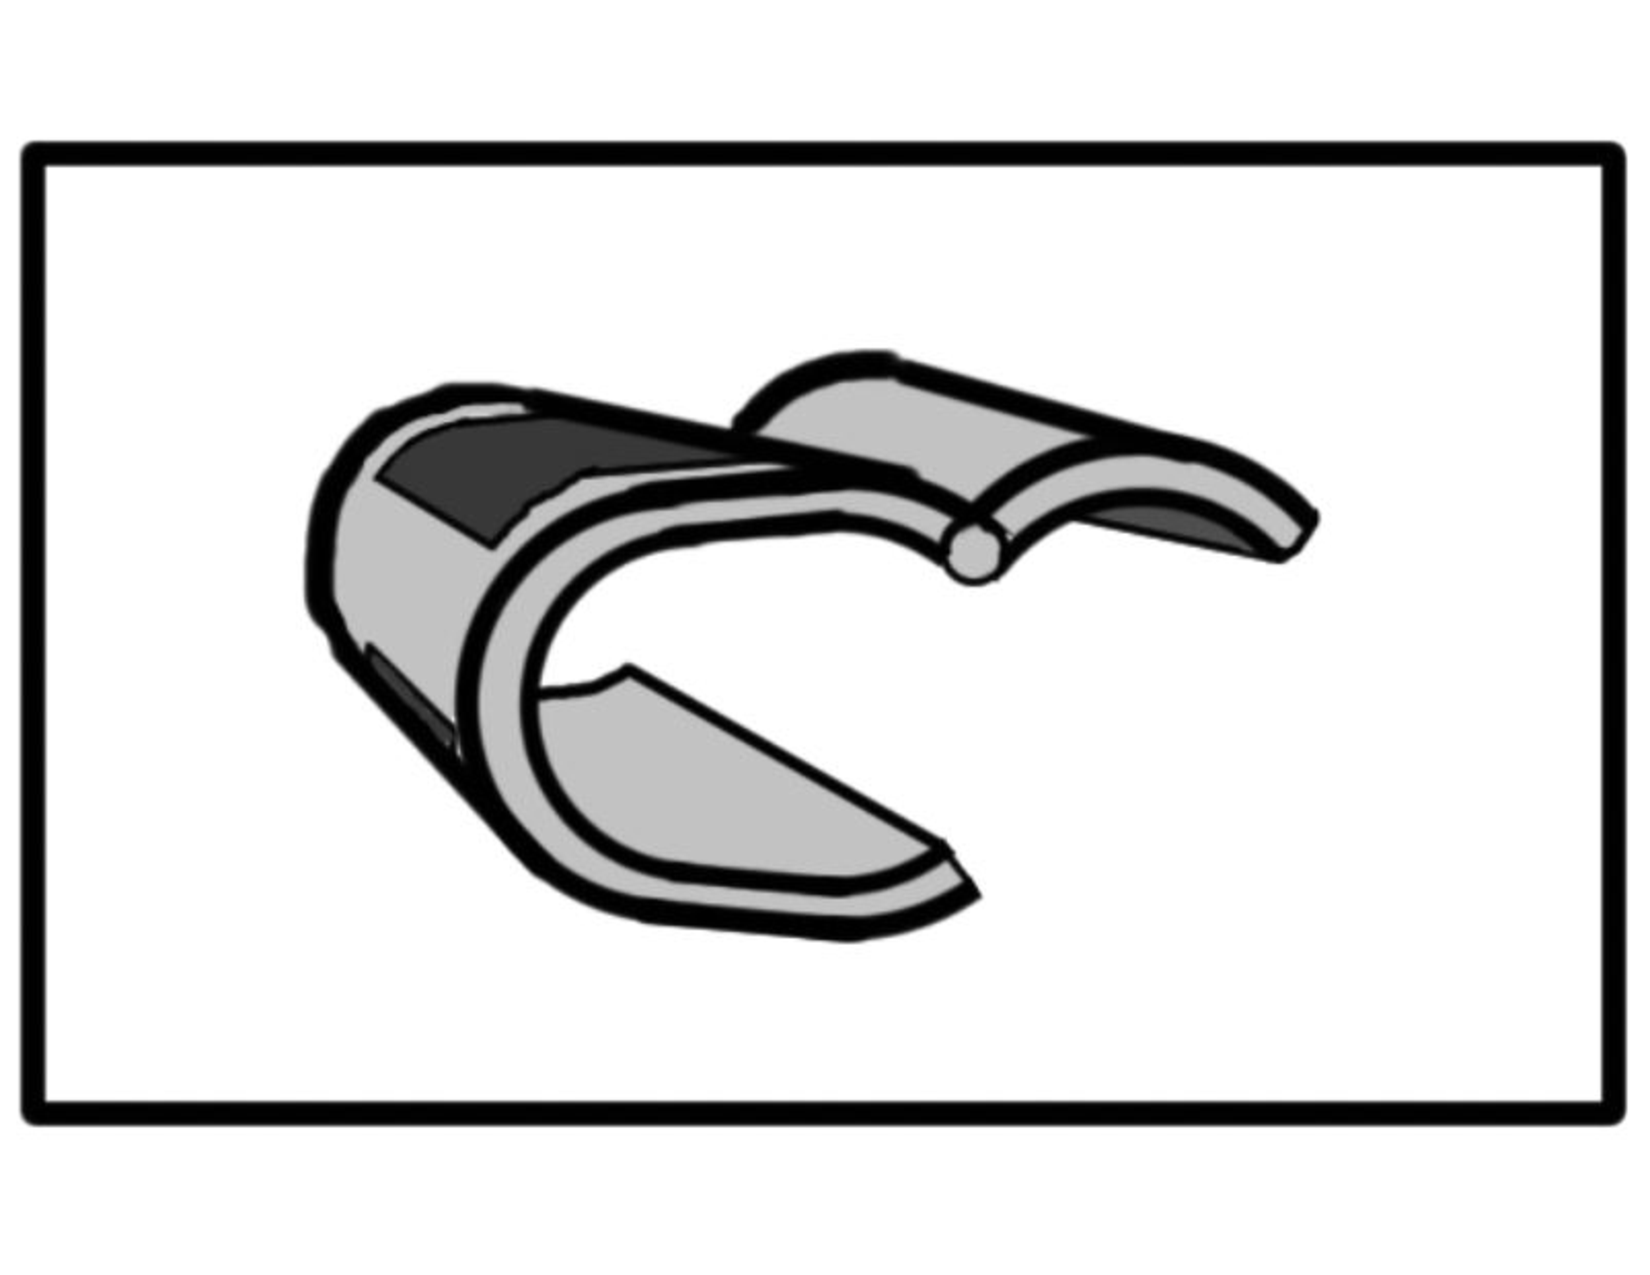
\includegraphics[width=4in]{device.pdf}       
   \caption{Device with hinged part open}
   \label{fig:device}
\end{figure}
\begin{figure}[H] %  figure placement: here, top, bottom, or page
   \centering
   \includegraphics[width=5in]{devicearm.png}   
   \caption{Top and bottom view of device as worn on left forearm. It shows position of features such as Sleep/Wake button(A), Brightness Control Buttons(B), and Camera(C)}
   \label{fig:deviceOnArm}
\end{figure}

\subsection{Screens}

The device has two screens, although only one screen will be active at any given time. The device would have multitouch capability to support familiar gestures such as pinching and rotating. These gestures have become staples in modern devices such as tablets and smartphones. With the use of gyroscopes and accelerometers, the device is able to detect its orientation and active the screen that is most appropriate.  The main screen appears on the top of the users forearm, on the same side most people wear their watches. The secondary screen is found on the bottom part of the forearm and will be visible whenever the users palm is oriented towards the user's face.

Most users are used to looking at the top of their forearm when interacting with wrist-worn devices such as watches or fitness trackers. As such, the main screen is where the user will spend most of their time interacting with the device. The main screen only has a \textbf{horizontal orientation}, since physically it would be uncomfortable to hold the device vertically and look at the screen at the same time. The main screen is where notifications will appear for the user. The user will be able to casually glance at the main screen to see notifications, making the same gesture used by people who are checking their watch. When the user wishes to interact with the device, the user can wake the device by pressing the Sleep/Wake button and unlocking the device. While interacting with the main screen, the user still looks at the device as if checking a watch. 

The secondary screen is almost identical to the main screen. However, the constraint of the arm make it difficult for a user to hold their arm in such a way to see the secondary screen in a horizontal orientation. As a result, the secondary screen is limited to only a \textbf{vertical orientation}. Users will use the secondary screen when they wish to view something in the upright position or if they wish to use the device's camera as a front-facing camera. 

The device has the menu interface that exists in tablets and smartphones. The main screen as well as the secondary screen have on-screen buttons which have a Back button, Home Button, and Search Button. When it came time to choose between capacitive and on-screen buttons, the design choice became on-screen for two reasons. One, since the the device two large screens, each one would need a set of capacitive buttons which would complicate the design. Two, capacitive buttons are always on, which make users prone to accidentally hitting the buttons when viewing videos or pressing buttons which are very close to the capacitive buttons. On-screen buttons, on the other hand, can be customized by users and positioned wherever the user chooses. This would allow right-handed and left-handed users to use the device with the same ease. In fact, the device's settings can be changed for right-handedness and left-handedness. In this way, the device would be as accessible to as many people as possible.

\subsection{Hardware Buttons}
The device has only three buttons. These are always found on the side of the device which faces the user's wrist. Most watches and wristwork devices already have buttons on the side of the device, so my design takes advantage of the cultural affordances associated with wrist-worn objects. The device has a Sleep/Wake button and two brightness buttons which are used to calibrate the brightness of the device, as pictured in Figure~\ref{fig:buttons}. I chose this based on the physical constraint of using the device where only one hand is available. It is much easier for the opposite hand to access the side of the device closest to the wrist. It is much more comfortable for the user to access buttons this way, and doing so does not obstruct the screen, which is important when the user is trying to calibrate the screen's brightness. 

\begin{figure}[H] %  figure placement: here, top, bottom, or page
   \centering
   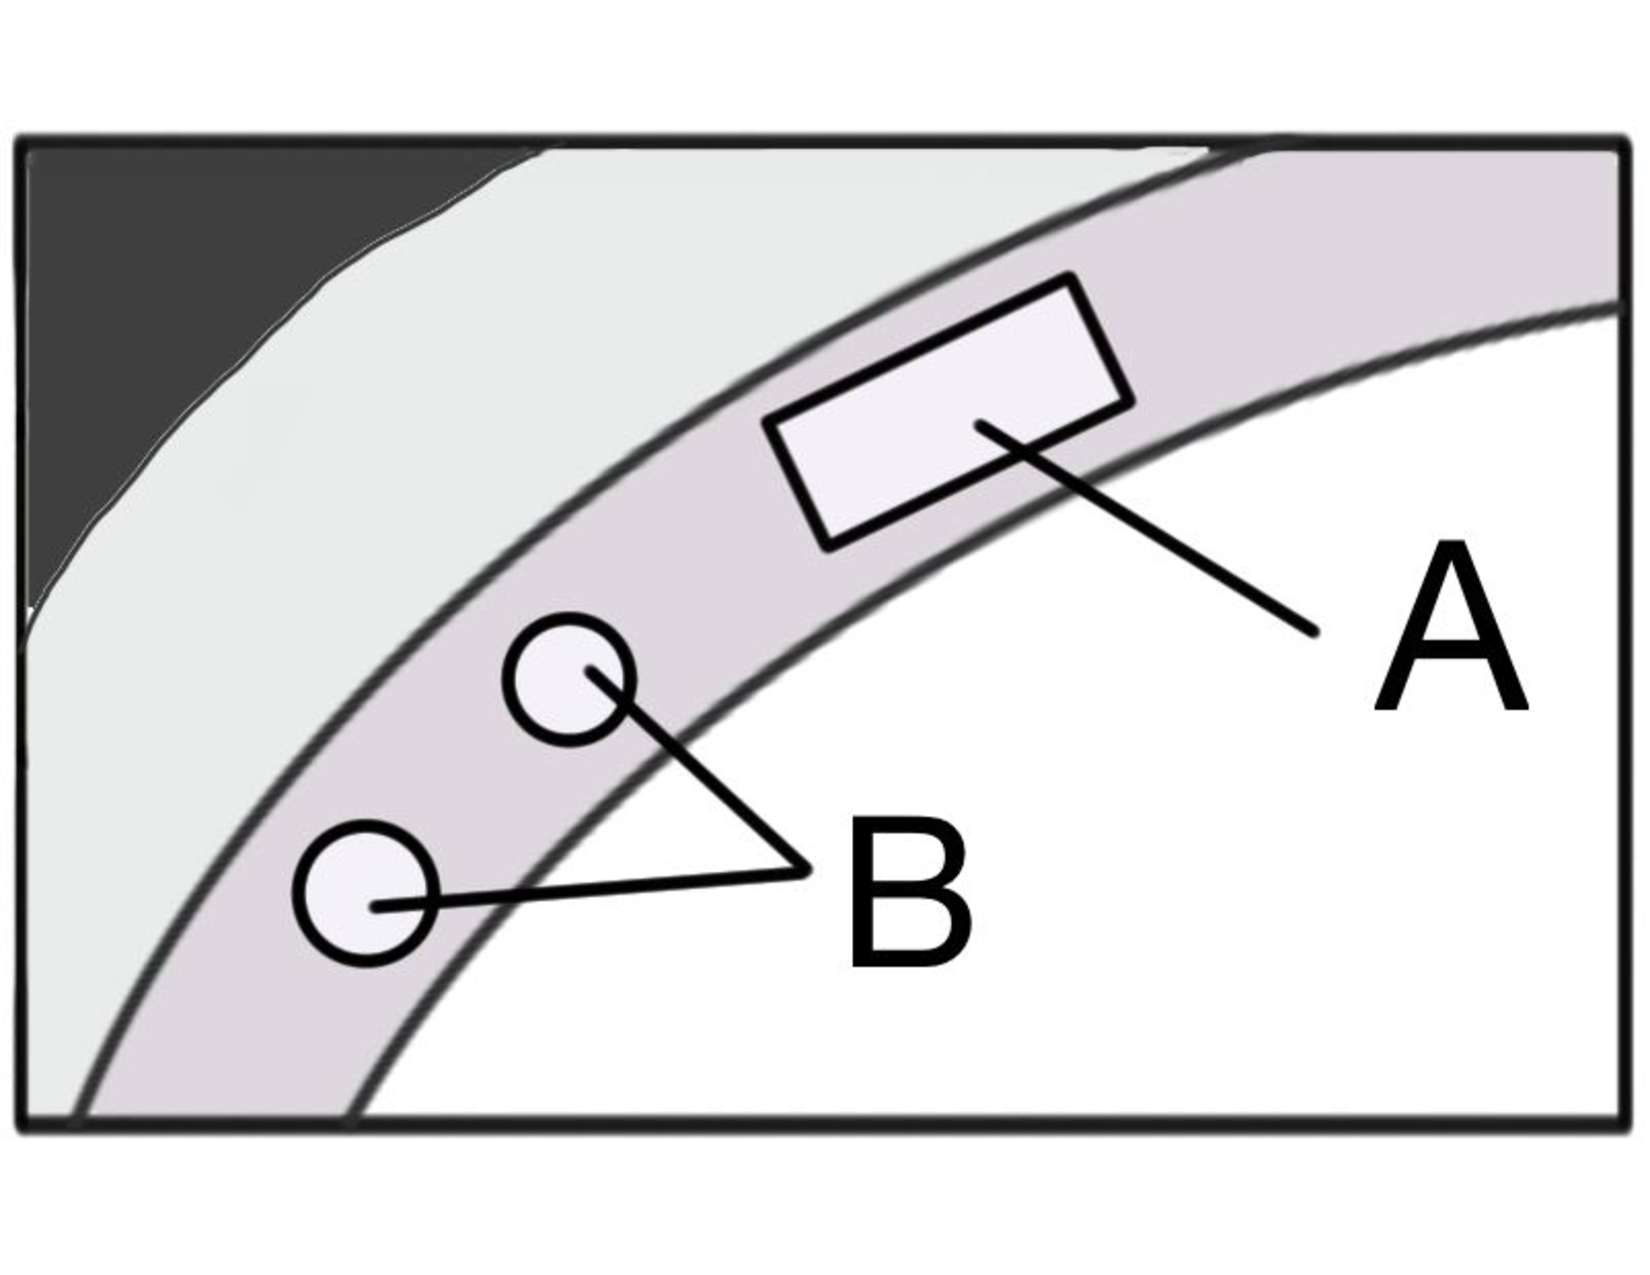
\includegraphics[width=3in]{buttons.pdf}   
   \caption{Close-up revealing sides of device. The Sleep/Wake button(A) and Brightness Control Buttons(B) are visible.}
   \label{fig:buttons}
\end{figure}

The design of using hardware buttons came from need to having buttons for actions that must by easily accessible regardless of the state of the device. The choice for the Sleep/Wake button is obvious; all portable devices(to the best knowledge of the author) make use of this button. The brightness of the screen is equally important, especially in the case of a wearable device. In most, if not all, smartphones and smartwatches, the brightness settings can only be adjusted from the user's screen. That is, if the user needs to make the screen brighter because he has trouble seeing the screen, he must first navigate through the devices menus, go to the brightness settings, and then change the brightness. This is, frankly, ridiculous. By making the brightness of the screen accessible from two hardware buttons, the user can change the brightness of the screen at any moment without actually interacting with the screen itself.

The brightness buttons swap functions depending on the handedness of the individual. There is no confusion between the brightness buttons and the Sleep/Wake buttons due to their difference in shape. However, in order to stay consistent with the affordance of higher buttons meaning increase and lower buttons meaning decrease, the function of the brightness buttons must change depending on the arm on which the user is wearing the device. Obviously, the brightness button furthest from the interior of the users arm increases the brightness of the screen, while the button closest to the interior decreases the brightness.

\section{Usage Scenarios}
\subsubsection{Notifications}
Most smartwatches serve to send users notifications from their phones. This device can also alert the user to notifications on the main screen. When the device receives a notification, it vibrates twice in rapid succession in order to alert the user. However, the device will not wake up until it perceives that the user is looking at it. It does this by using its accelerator and gyroscope to detect if the user is holding their hand as if looking at their a watch. This is so the device is the least intrusive as possible. In this way, the device won't flash possibly sensitive information to other people. Once the user is looking at the device, the main screen becomes active and shows a queue of notifications that the user hasn't seen (Figure~\ref{fig:notifications}). If the user wishes, they can dismiss notifications by pressing the white x on the notification. If the user wishes to unlock the device, she can drag the key icon towards the lock on the other side of the screen and unlock the device. This lock screen is the same screen that a user sees right after Waking the device using the Sleep/Wake button. The only difference is that the the screen automatically activates when the device receives a notification. 

\begin{figure}[H] %  figure placement: here, top, bottom, or page
   \centering
   \includegraphics[width=3in]{notifications.pdf}   
   \caption{Sample of what notification/lock screen.}
   \label{fig:notifications}   
\end{figure}

\subsubsection{Texting}
My proposed device borrows heavily from modern smartphones. One of the ways that my device borrows heavily from pre-existing software is the way that my device manages text input. My device will make use of the Go keyboard. The most important factor for choosing Go is that GO requires only a single finger in order to type in text. Users of the device can only use one of their hands. Go keyboards offer a decent degree of accuracy(9.6\%), has a high efficiency(14.18 words per minute) and have a high degree of user satisfaction(SUS score of 74)\cite{textInputSurvey}.

Users would navigate to the texting application and use the texting application the same as if it were a smartphone. The beauty of making a device so similar to a smartphone, one of the most successful consumer devices on the market, is that many of the tasks that users are familiar with now easily carry over on to my proposed device. Currently, the fastest text-input for smartwatches makes use of Zoomboard, achieving "roughly 10 words per minute"\cite{zoomboardVerdict}. A larger screen means that users have a greater degree of accuracy and speed.

\section{Issues}

Although my proposed device presents advantages over typical smartwatches in the market right now, it still faces some issues. Some of the most important issues arise out of the size of the wearable, its defining characteristic. A larger device is heavier, less discrete, and could be more uncomfortable \cite{WhyUsersDont}. It would be important to focus on using light, durable materials to prevent injury to the user. The surface area and the computational stress on the device could also make it prone to heating, which would increase discomfort and possibly risk injury to the user \cite{UserAcceptance}. 

Typical smartwatches take advantage of the cultural affordance in the familiarity of the shape of a watch. My design is relatively exotic in comparison. As such, the device is immediately noticeable. It is hard to hide a device that is the size of your arm. The current design is based off of the long forearm sleeve used by athletes such as basketball players. These sleeves are large and noticeable but stylish. However, some aesthetic improvements could possibly help to make the design more appealing. 

Another issue worth taking into consideration is the size of the screens and the propensity of getting cracked, scratched, or otherwise damaged. Since curved screens are so relatively new, it is difficult to predict whether or not they'll exhibit the same amount of durability as flat screens(my prediction is that the curved screens are more prone o damage). Each screen could be sold with a durable screen protector in order to minimize potential damage. Another important issue is making the device waterproof. It is unacceptable if a user is unable to use their device in the rain or if their device becomes permanently damaged due to the rain. This is because of the nature of wearables in general, as well as the large size of the wearable itself. Small wearables such as Google Glass or smartwatches could be easily put away in the users pockets. However, my devise is very large and it is unfeasible to remove the device unless one has a large briefcase or backpack to put the device in during a rainstorm. While it is possible to assume that users would exercise greater caution given the fact that they are wearing an expensive accessory on their arm, the nature of the wearable would cause users to become so accustomed to the wearable that they would in fact forget it's there. This brings us to the last and possibly the most important issue that this wearable faces. Price.

This wearable is rather large, probably larger than most smartphones out in the market right now. Arguably, this wearable could prove to twice as expensive than a high-end smartphone. Price alone might be a deterrent for users to adopt this wearable device. While there is always a number of individuals who would take interest on the device simply on novelty, we could not depend on novelty alone to appeal to users. This is difficult to compromise since the device must be made of strong, durable material as well as contain more electronics than a typical wearables. I believe that this device would probably be the most expensive wearable device on the market. It is possible to focus the product as a high end product, but this would definitely affect the accessibility of the product.

\section{User Response Predictions}
I believe that my device will rate very highly in all of Nielsen's usability metrics except possibly satisfaction. I say this because my device borrows very heavily from familiar smartphone interfaces and designs. To recap, here is a list of Nielsen's usability metrics:

\begin{itemize}
  \item Learnability (the time it takes to learn an interface)
  \item Efficiency (the speed of performance)
  \item Errors (the rate of errors committed by the users)
  \item Memorability (how easily users retain information about the interface)
  \item Satisfaction (Does the user like the interface?)
\end{itemize} 
 
Since my device works similar to a smartphone, both learnability and memorability are taken care off. There's no need for a user to learn too much information about my design since it's all so familiar. The only significant innovation is the introduction of brightness buttons, and these I believe are intuitive enough that users will quickly pick up on how to use them. The simplicity of the new features mean that users would also retain the information easily. The large screen makes interacting with the device similar to interacting with a smartphone, and thus has roughly the same degree of errors as smartphones. Another advantage of the large screen is the increased efficiency of the interface when compared to other wrist-wearables. 

The metric that seems the most uncertain is satisfiability. Since this is a theoretical system, it is difficult to determine how popular or desirable this device is. It is my hope that the device would appeal to all the tech-junkies out there that love the idea of wearables and would like wearables to do as much as their smartphones can. The success of the wearable under the other metrics would help, although not guarantee, attain a high degree of satisfaction. It is possible that users look at the device and simply find it unappealing. A great marketing campaign would help increase the appeal of the device, but ultimately, the final verdict rests in the users. 

A recent study found that 33\% wearable users discard or stop using their wearable devices after only \textbf{a year} of using the device \cite{wearablesStopUse}. This was mostly because they no longer found the device appealing, the novelty of the device having worn off. It is my hope that if my dream design for an interface ever comes to fruition, the device won't be left unused in a drawer a year after it was purchased.

\section{Conclusion}

Modern wrist-wearables are greatly limited by their size and their shape. This affects their battery life, computational power, and, more importantly, the devices' interface. My proposed device is a wearable that combines the size and efficiency of a smartphone with the wearability of a wrist-worn device.

\bibliographystyle{unsrt}
\bibliography{\myreferences}

\end{document}  